\documentclass[conference]{IEEEtran}
\usepackage[T1]{fontenc}
\usepackage{amsmath,amssymb,graphicx,url}
\begin{document}
\title{A Water-Inventory Comparator for Steam-Engine Speed}
\author{\IEEEauthorblockN{vikas H R}\IEEEauthorblockA{Roll No. 23B2282\\ME319, IIT Bombay}}
\maketitle
\subsection*{Abstract}
This paper studies a water-based speed governor. An engine-driven pump feeds a tank, while a floating outlet removes water at a nominally constant rate. A change in tank level records accumulated speed error. Pressure across an inlet restriction supplies a second signal that responds directly to speed. A lever combines the signals to adjust the steam throttle. The resulting model has three states: speed, water inventory and throttle position. With the assumed parameters, the student-executed MATLAB simulation gives a 5.55\% peak speed departure and 10.43 s recovery after either \ensuremath{\pm}30\% load step. Its results agree with an independent Python calculation. The mechanism has not been built, and its originality and period construction remain to be checked.

\subsection*{I. INTRODUCTION AND ASSUMPTIONS}
When a machine is connected to a mill shaft, the extra load slows the engine. Disconnecting a machine has the opposite effect. The throttle must therefore change as the load changes. The objective here is to restore normalized speed w = 1 after load steps from 1 to 1.3 or 0.7, using only mechanical and fluid components. The assignment allows a local linear model and gives priority to originality [1]. The proposed arrangement is a design hypothesis; the calculations test its behavior under stated assumptions.

Assume a unidirectional shaft, regulated boiler pressure, cycle-averaged torque, flooded positive-displacement pumping, incompressible water, atmospheric tank pressure and negligible bellows inertia. Lever and valve motion are locally linear. Float loading, pump slip, backlash and steam-chest delay are initially neglected and must be measured. All numerical parameters are design estimates; no prototype or engine data were obtained.

Brass or iron cylinders, check valves, copper pipe, leather bellows, floats, weights and pin-jointed levers are proposed period-compatible components. Pumping machinery existed before the target era [3]; this does not prove availability or adequacy of every proposed detail. No modern elastomers, electronics or precision electronic reference is assumed.

\subsection*{II. CONCEPTUAL DESIGN}
The shaft drives two phased reciprocating water pumps from a lower sump. Mean delivery q tracks shaft speed. Water crosses a restriction into an open tank. A separate guided float carries a rigid outlet assembly with its atmospheric discharge a fixed vertical distance H below the water surface. This assembly must translate with the surface; a fixed discharge would instead produce level-dependent outflow. A sensing float measures tank level.

\begin{figure}[ht]\centering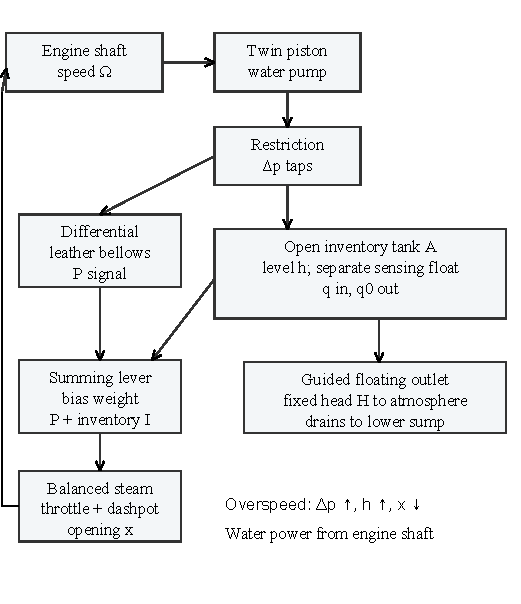
\includegraphics[width=\columnwidth]{../figures/mechanism.pdf}\caption{Fig. 1. Functional engineering schematic; routing and signs shown, not a dimensioned fabrication drawing.}\end{figure}
A differential bellows senses pressure on both sides of the inlet restriction, rejecting changes in tank static head when taps are properly referenced. A preloaded spring subtracts the nominal pressure. Its displacement and the sensing float displacement act through a summing lever with a bias weight. The lever commands a nearly pressure-balanced throttle; a water dashpot provides an overdamped valve lag.

On a load increase, the shaft slows, inflow and restriction pressure fall, and the level declines. Both signals open the throttle. At restored speed the inflow again equals the constant outflow, while a persistent level shift holds the increased opening. Integral memory is the water inventory, not a rotating flyweight position.

The outlet must retain prime, discharge freely above the lower sump, and keep H fixed through its full stroke. A vented guided carrier and rigid copper siphon or equivalent submerged outlet are construction candidates. Tube routing, guide friction and priming have not been demonstrated.

\subsection*{III. NOVELTY AND HISTORICAL LIMITS}
Watt, Porter, Proell, Hartnell and Wilson-Hartnell mechanisms use rotating centrifugal masses with different gravity/spring/linkage arrangements. This proposal instead measures displacement-pump flow and stores error as stationary liquid inventory; changing a flyball geometry is not its design step. However, non-centrifugal sensing alone is insufficient evidence of originality.

Maxwell explicitly discusses integral-like correction, damping and Siemens liquid governors [2]. His Siemens example uses a rotating cup with screw/spring coupling. Our stationary tank, translating constant-head reference outlet and separate differential-pressure path differ from that described mechanism, but hydraulic comparison and accumulated-error regulation are established ideas. The candidate contribution is this particular physical interconnection. An exhaustive patent or literature search was not performed; priority and assignment-level originality are unverified.

Before accepting the concept, search pump-pressure speed governors, float governors, liquid governors, constant-flow apparatus and hydraulic PI regulators. Compare diagrams and energy paths, not merely names. Obtain instructor feedback if a close arrangement is found. A modern floating-siphon search lead was found but its full document was inaccessible; it is not treated as verified evidence here.

\subsection*{IV. PHYSICAL MODEL AND LINEARIZATION}
Let \ensuremath{\Omega} be dimensional shaft speed, Q displacement per radian including gearing, A effective tank storage area, h liquid level and q\ensuremath{{}_0} the reference outflow. Neglect slip initially. Conservation of volume and a gravity outlet give

\begin{equation}q=Q\Omega,\quad A\dot h=Q\Omega-q_0\end{equation}
\begin{equation}q_0=C_d a_0\sqrt{2gH},\quad \Omega_0=q_0/Q\end{equation}
Here H is constant because the discharge moves with the free surface. A changing discharge coefficient or H changes the regulated speed. The effective A includes float displacement and must be calibrated.

\begin{equation}\Delta p=\frac{\rho}{2}\left(\frac{q}{C_r a_r}\right)^2=\Delta p_0w^2\end{equation}
Equation (3) is a quasi-steady restriction model. Define f(w) = (\ensuremath{\Delta}p \ensuremath{-} \ensuremath{\Delta}p\ensuremath{{}_0})/(2\ensuremath{\Delta}p\ensuremath{{}_0}) = (w\ensuremath{{}^2} \ensuremath{-} 1)/2. Since f(1 + v) = v + v\ensuremath{{}^2}/2, its small-signal sensitivity is unity.

Use w = \ensuremath{\Omega}/\ensuremath{\Omega}\ensuremath{{}_0}, l = T\ensuremath{_{\mathrm{L}}}/T\ensuremath{_{\mathrm{L0}}}, v = w \ensuremath{-} 1, d = l \ensuremath{-} 1, u = x \ensuremath{-} x\ensuremath{{}_0} and z = A(h \ensuremath{-} h\ensuremath{{}_0})/q\ensuremath{{}_0}. The inventory z has units of time. A spring and dashpot valve balance yields c dx/dt + k(x \ensuremath{-} x\ensuremath{_{\mathrm{cmd}}}) = 0, hence \ensuremath{\tau} = c/k after reflecting forces to the same coordinate.

\begin{equation}\dot z=v,\quad \tau\dot u+u=-k_p f(w)-k_i z\end{equation}
A general engine balance is J d\ensuremath{\Omega}/dt = T\ensuremath{_{\mathrm{s}}}(x, \ensuremath{\Omega}) \ensuremath{-} B\ensuremath{\Omega} \ensuremath{-} T\ensuremath{_{\mathrm{L}}}. Locally, expand T\ensuremath{_{\mathrm{s}}} about equilibrium, with x\ensuremath{{}_0} = 0.6. Define M = J\ensuremath{\Omega}\ensuremath{{}_0}/T\ensuremath{_{\mathrm{L0}}}, D = [B \ensuremath{-} \ensuremath{\partial}T\ensuremath{_{\mathrm{s}}}/\ensuremath{\partial}\ensuremath{\Omega}]\ensuremath{\Omega}\ensuremath{{}_0}/T\ensuremath{_{\mathrm{L0}}}, and K = (\ensuremath{\partial}T\ensuremath{_{\mathrm{s}}}/\ensuremath{\partial}x)/T\ensuremath{_{\mathrm{L0}}}. Then

\begin{equation}M\dot v=-Dv+Ku-d\end{equation}
Together (4)-(5) are a nonlinear pressure-sensing model; replacing f(w) by v gives the LTI model. The torque law itself is a local constitutive approximation, not a universal nonlinear steam-engine model. All states are perturbations from the same nominal equilibrium, initially zero.

\begin{equation}G_p(s)=\frac{K}{Ms+D}\end{equation}
\begin{equation}G_c(s)=\frac{k_p+k_i/s}{\tau s+1}\end{equation}
The controller includes valve dynamics. For error e = r \ensuremath{-} v, u = G\ensuremath{_{\mathrm{c}}}e; simulations use r = 0. The conceptual reference r represents a coordinated adjustment of flow reference and pressure bias, not an independently implemented automatic reference actuator.

\begin{equation}P(s)=\tau Ms^3+(M+\tau D)s^2\end{equation}
\begin{equation}{}+(D+Kk_p)s+Kk_i\end{equation}
\begin{equation}\frac{V}{R}=\frac{K(k_ps+k_i)}{P(s)}\end{equation}
\begin{equation}\frac{V}{D_L}=\frac{-s(\tau s+1)}{P(s)}\end{equation}
\begin{equation}\frac{U}{D_L}=\frac{k_ps+k_i}{P(s)}\end{equation}
D\ensuremath{_{\mathrm{L}}}(s) denotes the transform of load perturbation d, distinct from damping D. The load acts after the throttle; multiplying it by the throttle plant would give an incorrect disturbance transfer function.

\begin{figure}[ht]\centering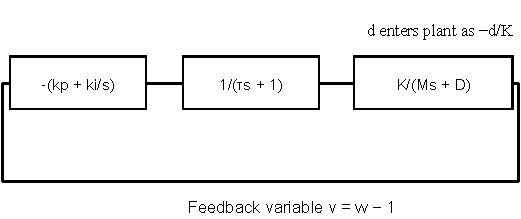
\includegraphics[width=\columnwidth]{../figures/feedback.pdf}\caption{Fig. 2. Controller and valve feed the engine; load enters the torque balance independently.}\end{figure}
\subsection*{V. PARAMETER SELECTION AND AUTHORITY}
Select M = 5 s, D = 1, K = 2, \ensuremath{\tau} = 0.5 s, k\ensuremath{_{\mathrm{p}}} = 2 and k\ensuremath{_{\mathrm{i}}} = 0.5 s\ensuremath{{}^{-1}}. These yield moderate proportional authority and deliberately slow integral correction. They are illustrative estimates chosen for feasibility and stability, not fitted values or a performance optimum.

One dimensional interpretation uses \ensuremath{\Omega}\ensuremath{{}_0} = 2\ensuremath{\pi} rad/s (60 rpm), T\ensuremath{_{\mathrm{L0}}} = 100 N m and J = 79.6 kg m\ensuremath{{}^2}, giving M = 5 s. A flywheel with mass concentrated at radius 0.8 m would require about 124 kg. A local steam torque law T\ensuremath{_{\mathrm{s}}}/T\ensuremath{_{\mathrm{L0}}} = 1.2 + 2u \ensuremath{-} 0.8v and B\ensuremath{\Omega}\ensuremath{{}_0}/T\ensuremath{_{\mathrm{L0}}} = 0.2 gives D = 1. The assumed torque-speed slope accounts for most damping and is especially important to measure.

Choose q\ensuremath{{}_0} = 10\ensuremath{{}^{-4}} m\ensuremath{{}^3}/s (6 L/min), Q = 1.59\ensuremath{\times}10\ensuremath{{}^{-5}} m\ensuremath{{}^3}/rad and A = 0.01 m\ensuremath{{}^2}. Thus q\ensuremath{{}_0}/A = 0.01 m/s and z = (h \ensuremath{-} h\ensuremath{{}_0})/0.01 m s\ensuremath{{}^{-1}}. Mean pump delivery is 100 mL/revolution; two phased plungers reduce ripple. At H = 0.2 m and C\ensuremath{_{\mathrm{d}}} = 0.6, the reference outlet diameter is about 10.4 mm.

Select \ensuremath{\Delta}p\ensuremath{{}_0} = 500 Pa. A 0.01 m\ensuremath{{}^2} differential bellows sees a 5 N nominal preload. A 100 N/m sensing spring produces 0.1 m displacement per unit v near nominal. With 20 mm full valve travel and 0.4 displacement ratio this gives k\ensuremath{_{\mathrm{p}}} = 2. Subtract the nominal bias with a weight or spring. These are local lever gains, not a completed force-balanced assembly.

The inventory branch needs valve travel / level travel = 1, because 20 mm \ensuremath{\times} k\ensuremath{_{\mathrm{i}}} \ensuremath{\times} A/q\ensuremath{{}_0} = 1. A 0.005 m\ensuremath{{}^2} sensing float has buoyancy stiffness about 49 N/m; a 3 mm relative immersion gives only 0.147 N. This is marginal authority: measured throttle and linkage resistance must be well below this scale. Any float immersion caused by linkage load corrupts the stored-error reading. A balanced valve, large float, counterweights or a carefully modeled pilot stage may be needed; a pilot stage would add dynamics absent here.

\subsection*{VI. STABILITY AND STEADY STATE}
For positive M, D, K, \ensuremath{\tau}, k\ensuremath{_{\mathrm{p}}} and k\ensuremath{_{\mathrm{i}}}, the cubic Routh first column is

\begin{equation}\tau M,\quad M+\tau D,\end{equation}
\begin{equation}\frac{(M+\tau D)(D+Kk_p)-\tau MKk_i}{M+\tau D},\end{equation}
\begin{equation}Kk_i\end{equation}
Strict positivity is necessary and sufficient. Therefore

\begin{equation}0<k_i<\frac{(M+\tau D)(D+Kk_p)}{\tau MK}\end{equation}
\begin{equation}P(s)=2.5s^3+5.5s^2+5s+1\end{equation}
The allowable k\ensuremath{_{\mathrm{i}}} is below 5.5 s\ensuremath{{}^{-1}}. The selected 0.5 s\ensuremath{{}^{-1}} gives a Routh column 2.5, 5.5, 4.54545, 1. Numerical poles are \ensuremath{-}0.270676857 and \ensuremath{-}0.964661572 \ensuremath{\pm} 0.739733011i, all in the left half-plane. The slow real pole dominates the recovery tail. For the complex pair only, \ensuremath{\omega}\ensuremath{_{\mathrm{n}}} = 1.21564 rad/s and \ensuremath{\zeta} = 0.793543. A single second-order damping ratio does not characterize this entire loop.

For constant d and a stable unsaturated loop, dz/dt = 0 implies v\ensuremath{\infty} = 0. Equations (4)-(5) then give u\ensuremath{\infty} = d/K and z\ensuremath{\infty} = \ensuremath{-}d/(Kk\ensuremath{_{\mathrm{i}}}). At d = \ensuremath{\pm}0.3 the throttle settles to 0.75 or 0.45; the level shifts by \ensuremath{\mp}3 mm. The water inventory can hold a new throttle position with no sustained speed error.

With the governor disconnected and throttle fixed, v(t) = \ensuremath{-}(d/D)[1 \ensuremath{-} exp(\ensuremath{-}Dt/M)]. Thus the steady speeds are 0.7 and 1.3; the pole is \ensuremath{-}0.2 s\ensuremath{{}^{-1}}. Open-loop settling to a displaced equilibrium is not recovery to nominal speed.

A finite parameter check of all 64 independent \ensuremath{\pm}20\% corners of M, D, K, \ensuremath{\tau}, k\ensuremath{_{\mathrm{p}}}, k\ensuremath{_{\mathrm{i}}} was stable; the smallest decay margin was 0.1446 s\ensuremath{{}^{-1}}. This is a finite sweep, not a proof for arbitrary uncertainty or omitted delays. A deliberate k\ensuremath{_{\mathrm{i}}} = 12 s\ensuremath{{}^{-1}} example produces unstable poles 0.27264 \ensuremath{\pm} 1.85002i, demonstrating the finite tuning boundary.

\subsection*{VII. SIMULATION PROTOCOL AND RESULTS}
The code integrates the three LTI state equations with classical RK4 at 0.01 s for 60 s, with steps at t = 0. Figures show the first 30 s. The MATLAB/Octave implementation uses base operations and independently compares every sample with a matrix-exponential solution. The student ran the supplied script in MATLAB and provided the output CSVs, plots and completion screenshot. The MATLAB peak values, settling times and throttle extrema agree with the independent Python results within 10\ensuremath{{}^{-9}}. The MATLAB release was not recorded; Octave was not tested.

Python verification compared RK4 with an eigenmode closed-form solution (maximum state difference 2.26\ensuremath{\times}10\ensuremath{{}^{-11}}), halved the time step (difference 2.12\ensuremath{\times}10\ensuremath{{}^{-11}}), and verified equal-and-opposite perturbations for the two steps. MATLAB also compared RK4 with its matrix-exponential solution, with maximum state error 2.251\ensuremath{\times}10\ensuremath{{}^{-11}} in each load case. These checks establish numerical consistency of the assumed model, not physical validation.

\begin{figure}[ht]\centering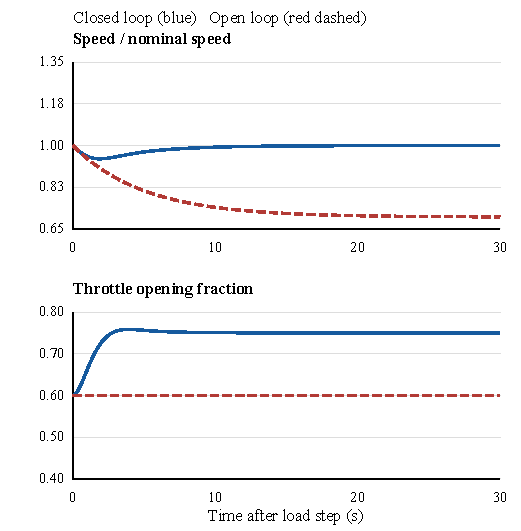
\includegraphics[width=\columnwidth]{../figures/increase.pdf}\caption{Fig. 3. Load increase 1 \ensuremath{\to} 1.3. Student-executed MATLAB trace, independently checked against Python.}\end{figure}
The increased load initially gives dv/dt = \ensuremath{-}0.3/5 = \ensuremath{-}0.06 s\ensuremath{{}^{-1}}. Speed reaches 0.944482 at 1.89 s and then approaches 1. The throttle briefly peaks at 0.758722 before settling to 0.75. At 60 s the computed speed is 0.999999991. Open-loop speed approaches 0.7 while the throttle stays at 0.6.

\begin{figure}[ht]\centering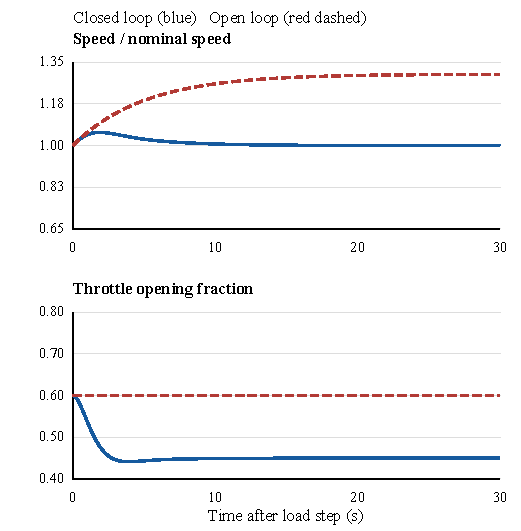
\includegraphics[width=\columnwidth]{../figures/decrease.pdf}\caption{Fig. 4. Load decrease 1 \ensuremath{\to} 0.7. Student-executed MATLAB trace; linear symmetry reverses the deviations.}\end{figure}
The decreased load reaches speed 1.055518 at 1.89 s; throttle reaches a minimum of 0.441278 before settling to 0.45. At 60 s the computed speed is 1.000000009. Open-loop speed approaches 1.3.

For both closed-loop cases, the maximum absolute speed departure is 5.5518\% of nominal, or 18.506\% of the 0.3 load-step magnitude under unit-normalized comparison. Define settling as remaining within \ensuremath{\pm}0.006 of the appropriate final speed, using 2\% of the disturbance magnitude rather than 2\% of nominal speed. The closed loop settles in 10.43 s; open loop settles to its displaced equilibrium in 19.57 s. Sample resolution is 0.01 s.

There is no sampled crossing of nominal speed: recovery overshoot, defined as excursion across nominal divided by |d|, is zero. This is different from the initial 5.55\% underspeed/overspeed excursion. Throttle remains inside [0,1], so actuator limits are not active in these LTI cases.

Retaining f(w) = (w\ensuremath{{}^2} \ensuremath{-} 1)/2 in an additional RK4 check changes speed by at most 0.001004 for the load increase and 0.000956 for the decrease relative to the LTI traces. This modest local sensor correction does not validate a full nonlinear engine or friction model. The open-loop \ensuremath{\pm}30\% speed departures are larger than the closed-loop departures and make its local torque approximation less reliable.

\subsection*{VIII. PRACTICAL LIMITS AND VALIDATION}
The reference water flow is the speed standard. Pump slip and outlet calibration errors shift that standard: \ensuremath{\Omega}\ensuremath{\infty} = q\ensuremath{_{\mathrm{out}}}/Q\ensuremath{_{\mathrm{eff}}}. A 1\% reference flow error therefore causes approximately 1\% speed bias if Q is unchanged. A fixed outlet or parasitic level-dependent leak adds a term \ensuremath{-}\ensuremath{\lambda}z to dz/dt and removes ideal integral regulation. With dz/dt = v \ensuremath{-} \ensuremath{\lambda}z, the steady error is v\ensuremath{\infty} = \ensuremath{-}d/[D + Kk\ensuremath{_{\mathrm{p}}} + Kk\ensuremath{_{\mathrm{i}}}/\ensuremath{\lambda}] for \ensuremath{\lambda} > 0.

Float drag, meniscus forces, backlash, water contamination and valve stiction can create deadbands and limit cycles absent from the linear model. Slosh and plunger ripple can excite the lever; phased plungers, a baffled tank and low-mass floats reduce these effects but their added dynamics must be measured. Bellows or connecting-pipe lag is omitted; stability of the present cubic cannot be assumed after adding it.

Priming loss or blockage changes outflow abruptly. An empty/full tank bounds the integrator and can leave the throttle at a limit. Provide visible level marks, travel stops, overflow return to the sump, a manual shutoff and independent overspeed trip. Those provisions are design requirements, not implemented or validated safety functions. Startup must establish prime, level h\ensuremath{{}_0} and nominal bias before automatic engagement.

At assumed total pump pressure rise 1.5 kPa, ideal hydraulic power is 0.15 W; real shaft power is higher by losses and pump efficiency. Nominal external load power is about 628 W. The small power estimate supports plausibility only. Verify the actual lift, restriction loss and throttle forces together. Do not infer valve authority from pump power alone.

With a full 20 mm valve stroke, \ensuremath{\pm}3 mm level adjustment provides only \ensuremath{\pm}3 mm valve movement, consistent with u\ensuremath{\infty} = \ensuremath{\pm}0.15. The mechanism drawing is functional: lever pivots, spring reaction loads, bellows common-mode balance, float displacement and minimum force margin still need a dimensioned free-body design. Significant redesign, especially a servo, requires a revised model and new stability analysis.

Recommended bench sequence: calibrate q versus \ensuremath{\Omega} and head; measure outlet flow versus h; measure bellows and float displacement under load; identify valve lag and torque gains; then test a water-powered surrogate before any steam application. Record uncertainties and repeat the \ensuremath{\pm}30\% disturbance tests with independently obtained parameters.

\subsection*{IX. CONCLUSIONS}
The model shows how tank level can retain the throttle adjustment needed after a load change, while restriction pressure provides a faster correction. For the chosen parameters, the Routh test and numerical solutions agree: the ideal loop is stable and returns to nominal speed after both specified load steps. The throttle remains within its available travel. These findings apply to the assumed model; they do not demonstrate that the proposed hardware will work.

The most useful feature is that the stored error can be seen directly as a change in water level. The main practical questions are whether the float can move the throttle with enough force and whether the floating outlet can hold a constant discharge. Measuring those quantities is the next design step. The prior-art comparison must also be extended. MATLAB execution and the numerical cross-check have been completed.

\subsection*{REFERENCES}
[1] P. Agarwal, ``Reinventing the Steam Engine Governor,'' ME319: Control Systems, Assignment 1, IIT Bombay, Autumn 2026, pp. 1-5. User-supplied assignment PDF; requirements inspected in full.

[2] J. C. Maxwell, ``On Governors,'' Proceedings of the Royal Society of London, vol. 16, pp. 270-283, 1868, doi: 10.1098/rspl.1867.0055. Original paper retrieved via University of Cambridge: https://www.damtp.cam.ac.uk/user/gold/pdfs/teaching/old\_literature/Maxwell1868.pdf (accessed Oct. 15, 2026). Used for historical similarities and dynamics context, not our numerical parameters.

[3] Science Museum Group, ``Newcomen Atmospheric Engine,'' collection object 1920-124/1, 1791 engine; catalogue describes first engine in 1712. https://collection.sciencemuseumgroup.org.uk/objects/co50900/newcomen-atmospheric-engine (accessed Oct. 15, 2026). Establishes period pumping context only.

\subsection*{REPRODUCIBILITY AND SUBMISSION STATUS}
Source code, parameter values, executed CSV traces, verified.json and build instructions accompany this draft. Repository URL: https://github.com/vikashr-alt/steam-governor. Author: vikas H R, Roll No. 23B2282. Repository files accompany this report.

The student completed MATLAB execution and supplied output files; these agree with the independent Python calculation. Octave compatibility has not been tested. No experiments, manufacturing feasibility certification, exhaustive originality verification, team contribution percentages or final submission are claimed. The confidential peer evaluation must reflect each student's actual contribution.

\clearpage\onecolumn
\section*{AI-Use Appendix}
\subsection*{Scope and tools}
This draft was prepared with the OpenAI Codex assistant in the desktop app. The exact underlying model identifier was not independently exposed and is not claimed. Tools actually used: Python 3 with NumPy for RK4, eigenvalues and checks; ReportLab for typesetting/vector figures; pdfplumber and PDF rendering for inspection; web search for limited primary-source comparison. The student executed the supplied script in MATLAB; output CSVs, plots and a completion screenshot were reviewed. The MATLAB release was not recorded. No symbolic algebra package or Octave run was used.
\subsection*{Prompt and use}
User prompt: ``Use the uploaded ME319 Assignment 1 PDF to help complete a rigorous, original steam-engine governor project. Develop and check an historically plausible novel concept, derive and verify control equations and stability, implement reproducible MATLAB/Octave simulations and plots for \ensuremath{\pm}30\% load, and prepare a maximum-six-page IEEE-style paper plus one-page honest AI-use appendix, repository-ready code and README. Clearly mark assumptions and anything requiring the student's own validation; do not fabricate originality verification, simulation results, citations, or GitHub URL.'' The assistant retrieved the assignment, proposed the mechanism, derived the model, wrote source files and drafted this report.
\subsection*{Accepted provisionally}
Conservation-of-volume inventory integration; differential-pressure proportional sensing; negative feedback sign; cubic characteristic polynomial; Routh condition; reproducible RK4 and analytic numerical checks. Engineering reasons: inventory preserves load-dependent throttle position at zero speed error, while proportional correction and valve damping avoid an undamped pure-integral loop. Selected gains satisfy the cubic stability test. The student executed the simulations and supplied the resulting files. Independent rederivation and physical validation remain outstanding.
\subsection*{Modified or rejected during preparation}
A fixed tank outlet was rejected as a basis for ideal integration because its flow varies with level. The proposal instead requires a translating constant-head outlet, whose feasibility remains unverified. Broad claims of novel hydraulic regulation were rejected after comparison with Maxwell/Siemens prior art. Initially unsupported execution claims were withheld; MATLAB execution is now documented by student-supplied outputs. Measured parameters, proven historical construction, complete physical validation is still not claimed. No experimental results were generated.
\subsection*{Validation actually completed}
Independent Python numerical integration agreed with an eigenmode solution within 2.26e-11 state units; halving the time step changed states by less than 2.12e-11. Opposite load steps had exact perturbation symmetry. A pressure-sensor nonlinear comparison and 64 parameter-corner check were executed. The student also ran MATLAB. Both cases gave a 1.89 s peak time and 10.43 s settling time; reported metrics matched Python within 1e-9, and the maximum MATLAB RK4/expm error was 2.251e-11. These checks test the assumed equations only, not physical feasibility or originality. The PDF was checked for page count and rendered layout.
\subsection*{Student / team actions still required}
MATLAB execution and output comparison are complete. Independently rederive equations; verify component chronology and perform broader prior-art comparison; dimension the lever and verify float/valve forces; calibrate parameters and test omitted dynamics. Author details have been added: vikas H R, 23B2282. The repository is https://github.com/vikashr-alt/steam-governor. Update this appendix with actual student changes and tools, and submit honest confidential peer evaluations. No contribution percentages, experimental validation or complete student engineering review are implied by this draft. This appendix must be revised if the final project differs.
\end{document}